\section{ADDITIONAL EXPERIMENTS}\label{sec:add_expes}

\subsection{Details of \textsf{glmnet} versus \textsf{SLOPE} Comparison}
\label{sec:slope-vs-glmnet}

In this experiment, we ran the \pkg{glmnet}~\parencite{friedman2022} and \pkg{SLOPE}~\parencite{larsson2022d} packages on the \dataset{bcTCGA} dataset, selecting the regularization sequence \(\lambda\) such that there were 100 nonzero coefficients and clusters at the optimum for \pkg{glmnet} and \pkg{SLOPE} respectively.
We used a duality gap of \(10^{-6}\) as stopping criteria.
The features were centered by their means and scaled by their standard deviation.
The code is available in the supplement.

\subsection{Study on Proximal Gradient Descent Frequency}
To study the impact of the frequence at which the pgd step in the \texttt{hybrid} solver is used, we performed a comparative study with the \dataset{rcv1} dataset.
We set this parameter to values ranging from $1$ \textit{i.e.}, the \texttt{pgd} algorithm, to 9 meaning that a pgd step is taken every $9$ epochs.
The sequence of $\lambda$ has been set with the Benjamini-Hochberg method and parametrized with $0.1 \lambda_{\text{max}}$.

\Cref{fig:pgd_freq} shows the suboptimality score as a function of the time for the different values of the parameter controlling the frequency at which a pgd step is going to be taken.
A first observation is that as long as this parameter is greater than $1$ meaning that we perform some coordinate descent steps, we observe a significant speed-up.
For all our experiments, this parameter was set to $5$ and was never changed.
We see on this figure that any choice of parameter between $3$ and $9$ would basically lead to the same performance.

\begin{figure*}[htb]
  \centering
  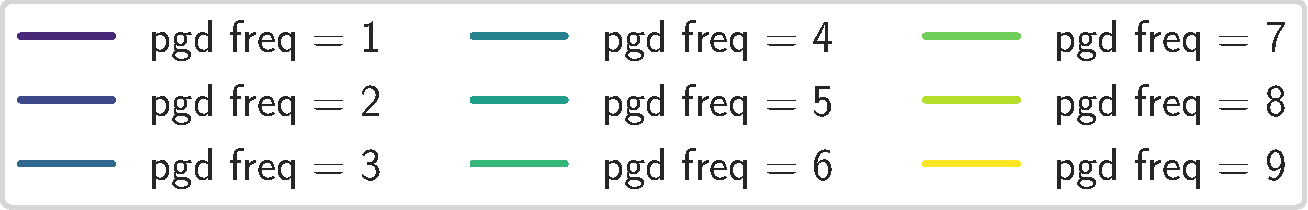
\includegraphics[scale=0.35]{pgd_freq_legend.pdf} \\
  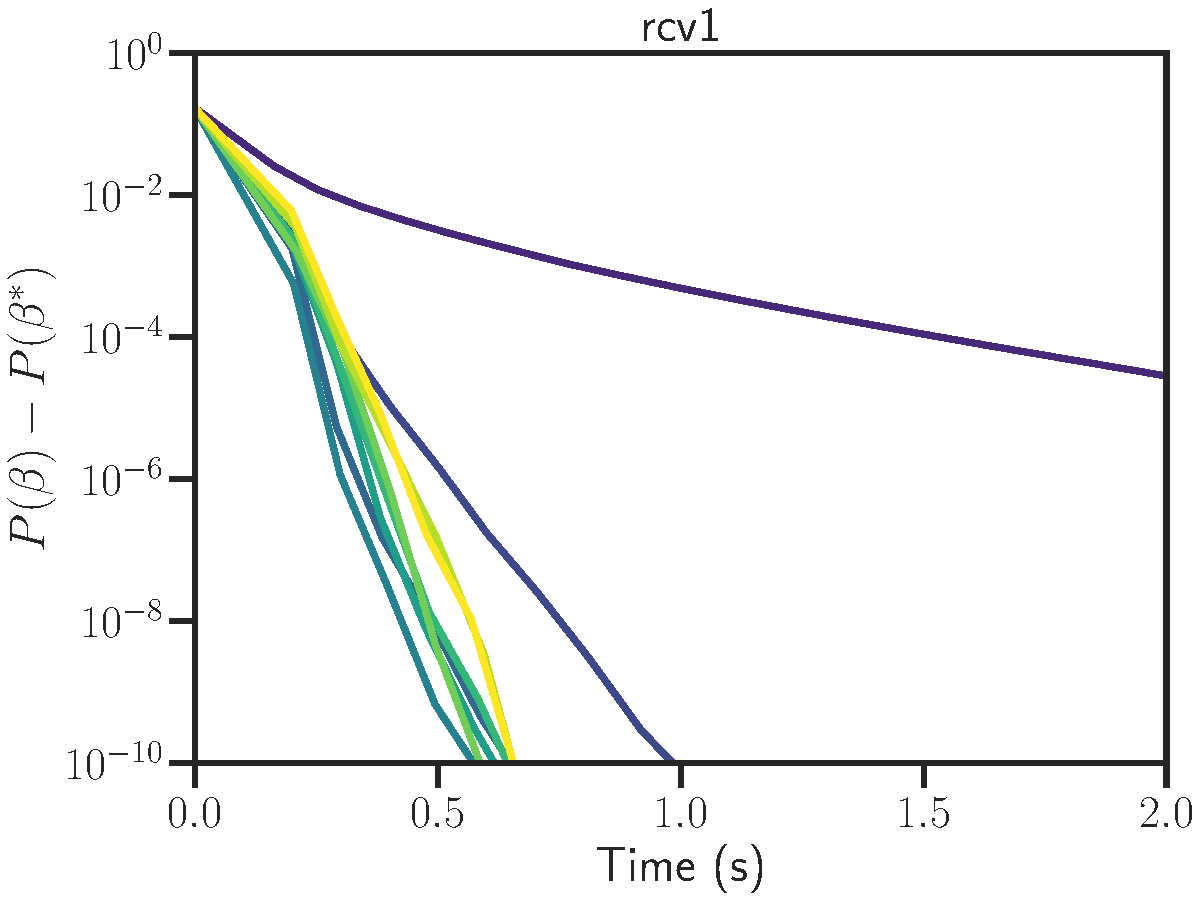
\includegraphics[scale=0.4]{pgd_freq.pdf}
  \caption{Suboptimality score as a function of the time for different frequency of PDG step inside the \texttt{hybrid} solver.}
  \label{fig:pgd_freq}
\end{figure*}

\subsection{Benchmark with different parameters for the ADMM solver}
\label{sec:admm-benchmarks}

We reproduced the benchmarks setting described in \Cref{sec:experiments} for the simulated and real data.
We compared the \texttt{ADMM} solver with our \texttt{hybrid} algorithm for different values of the augmented Lagrangian parameter $\rho$.
We tested three different values $10, 100$ and $1000$ as well as the adaptive method~\parencite[Sec. 3.4.1]{boyd2010}.

We present in \Cref{fig:simulated_appendix} and \Cref{fig:real_appendix} the suboptimality score as a function the time for the different solvers.
We see that the best value for $\rho$ depends on the dataset and the regularization strengh.
The value chosen for the main benchmark (\Cref{sec:experiments}) performs well in comparison to other \texttt{ADMM} solvers.
Nevertheless, our \texttt{hybrid} approach is consistently faster than the different  \texttt{ADMM} solvers.

\begin{figure*}[!t]
  \centering
  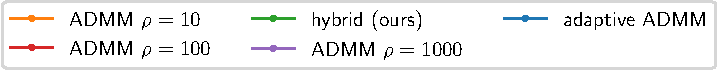
\includegraphics[scale=0.47]{simulated_legend_appendix.pdf}
  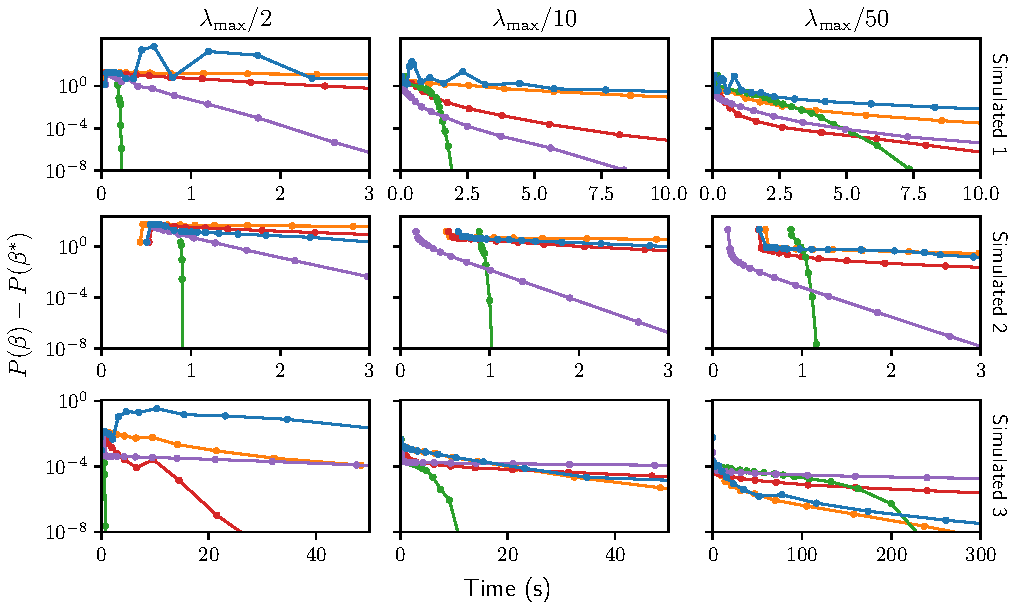
\includegraphics[scale=0.5]{simulated_appendix.pdf}
  \caption{\textbf{Benchmark on simulated datasets.} Suboptimality score as a function of time for SLOPE on multiple simulated datasets and for multiple sequence of $\lambda$.}
  \label{fig:simulated_appendix}
\end{figure*}


\begin{figure*}[!t]
  \centering
  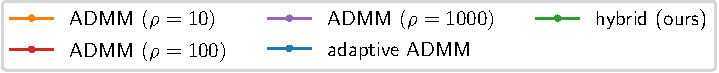
\includegraphics[scale=0.47]{real_legend_appendix.pdf}
  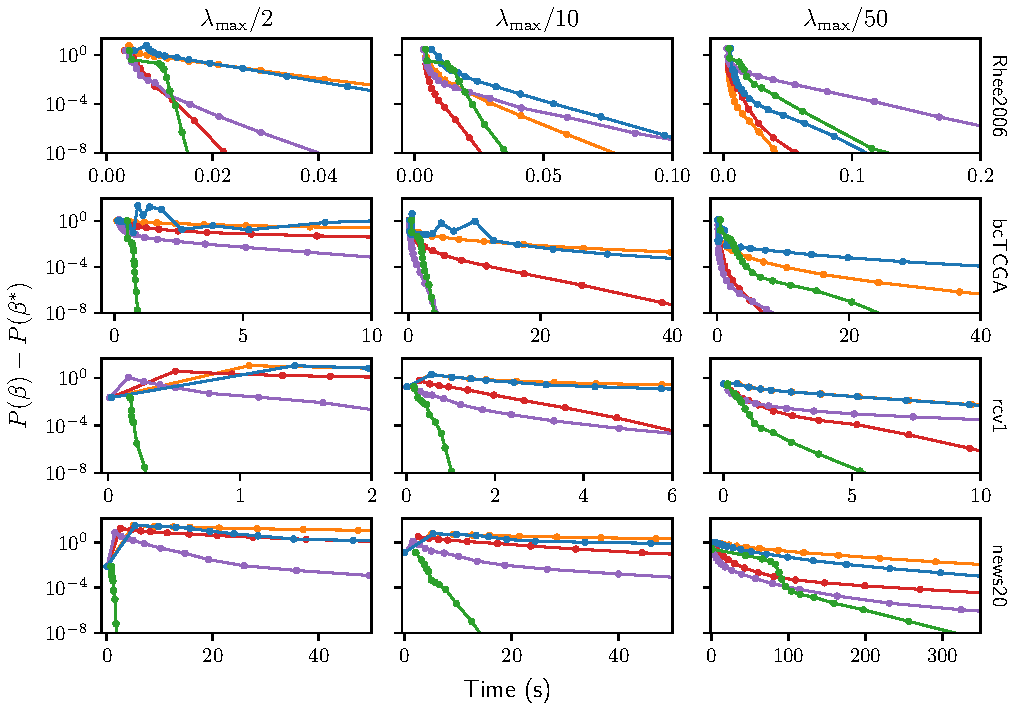
\includegraphics[scale=0.5]{real_appendix.pdf}
  \caption{\textbf{Benchmark on simulated datasets.} Suboptimality score as a function of time for SLOPE on multiple simulated datasets and for multiple sequence of $\lambda$.}
  \label{fig:real_appendix}
\end{figure*}
